\documentclass[10.7pt,a4paper]{letter} %EMW: I usually just switch to article so I can use refs, but up to you. 
\usepackage[top=.75in, bottom=.75in, left=.75in, right=0.75in]{geometry}
\usepackage{graphicx}
\usepackage{natbib}
%\address{1300 Centre Street \\ Boston, MA, 20131}

\begin{document}
\bibliographystyle{..//..//refs/bibstyles/amnat.bst}
\begin{letter}{}
\includegraphics[width=0.25\textwidth]{/Users/aileneettinger/Dropbox/Documents/Work/AA_heading.pdf}
\pagenumbering{gobble}

\opening{Dear Editor:}
Please consider our paper, `Spatial and temporal shifts in photoperiod with climate change' for publication as an `Opinion' in \emph{Global Change Biology}. It addresses a critical question in global change research: What are the implications of the altered photoperiod that plants and animals experience as they shift their ranges and seasonal activities with climate change? We use a synthesis of plant experiments that test effects of temperature and photoperiod on spring phenology (Wolkovich et al. 2019) to show how widespread and important photoperiod responses may be.

The two most-observed biological impacts of climate change are shifts in space (altitudinal, latitudinal range shifts) and time (phenological shifts, Poloczanska et al. 2013, Chen et al 2011, Parmesan et al 2006). Both alter the experienced photoperiod (Saikkonen et al 2012), which could dramatically affect performance and fitness. However, the magnitude of effects from shifts in photoperiod with climate change are unknown or unquantified for the vast majority of species.  We address this gap by quantifying expected changes in experienced photoperiod due to shifts in space versus time, given observations of spatial and temporal shifts to date (Chen et. al 2011, Parmesan and Yohe 2003), and put them in a novel, global context. We find that---despite a focus on photoperiod changes due to shifts in species distributions (e.g., Way and Montgomery 2015, Saikkonen et al 2012)---changes in experienced photoperiod due to temporal shifts appear to be orders of magnitude larger than those due to spatial shifts (e.g., 1.6 hours for expected temporal shifts versus one minute of change for spatial shifts). 

Our work is especially timely and important because it focuses on the intersection of photoperiod and spring phenology (as do the following recently published papers: Chamberlain et al 2019; Richardson, A.D., et al. 2018; Fu et al 2019)---an area of growing interest given recent studies suggesting photoperiod may underlie declining responses to warming. To date, the role of photoperiod has received far more detailed attention for end-of-season activities, such as growth cessation in the fall, than for spring activities. Though photoperiod cues dominate in the fall for many organisms, fall phenology responses to climate change have been muted. In contrast, spring phenology responds strongly to temperature and thus has advanced substantially with warming---causing cascading, and generally unexplored, effects on photoperiod experienced at the start of spring. We demonstrate that incorporating photoperiod into forecasts is possible by leveraging existing experimental data: as an example, we show that growth chamber experiments on woody plant spring phenology often have data relevant for climate change impacts %(e.g., Fig. 2). 
We highlight how new modeling approaches can improve predictions of when, where, and how much photoperiod is likely to affect future spring phenology and can be combined with new empirical work to advance our understanding of the role of photoperiod in a warming world. % (Wolkovich et al. 2019)

Our paper falls squarely within the scope of \emph{GCB}: climate change-induced shifts in photoperiod would have wide-reaching impacts on many plant and animal species. Photoperiod acts as a cue for the spring emergence and migration timing of diverse species, and alterations to experienced photoperiod can affect development, growth, and fitness for plants, insects, fish, and mammals, among other organisms. Thus, understanding these changes is critical for biologists forecasting species responses, policy-makers dependent on these forecasts for adaptation strategies, and those dependent on the services provided by these species. Yet, photoperiod has rarely been included in forecasts of responses to climate change and implications of climate-change-induced shifts in photoperiod are largely unexplored, especially for early-season spring events, where changes will be most dramatic. 
\\
\\
Co-authors are D. Buonaiuto, C. Chamberlain, I. Morales-Castilla, and E. Wolkovich. We suggest the following potential reviewers: Josep Pe\~nuelas, David Inouye, Ally Phillimore, and Mark Schwartz.
Thank you for considering our paper.

Sincerely,\\
\includegraphics[scale=.4]{/Users/aileneettinger/Dropbox/Documents/Work/AileneEttingerSignature.png} \\
\\
\begin{footnotesize}
Ailene Ettinger

NRC Research Associate, Northwest Fisheries Science Center

Visiting Fellow, Arnold Arboretum of Harvard University
\end{footnotesize}
\\
%\newpage
\\
\noindent \emph{References in letter}
\begin{footnotesize}

\item Chamberlain, C.J., et al. 2019. Rethinking false spring risk.  \emph{Global Change Biology}.

\item Chen, I.-C., et al. 2011. Rapid range shifts of species associated with high levels of climate warming.  \emph{Science}, 333:1024-1026.
\item Fu, Y.H., et al, 2019. Daylength helps temperate deciduous trees to leaf-out at the optimal time. \emph{Global change biology}.

\item Parmesan, C. and Yohe, G., 2003. A globally coherent fingerprint of climate change impacts across natural systems.  \emph{Nature}, 421:37.

\item Parmesan, C., 2006. Ecological and evolutionary responses to recent climate change.  \emph{Annu. Rev. Ecol. Evol. Syst.}, 37: 637-669.

\item Poloczanska, E. S., et al. 2013. Global imprint of climate change on marine life. \emph{Nature Climate Change}, 3: 919.

\item Richardson, A.D., et al. 2018. Ecosystem warming extends vegetation activity but heightens vulnerability to cold temperatures. \emph{Nature}, 560: 368.

\item Saikkonen, K., et al. 2012. Climate change-driven species' range shifts filtered by photoperiodism. \emph{Nature Climate Change}, 2:239.

\item Way, D. A., and R. A. Montgomery. 2015. Photoperiod constraints on tree phenology, performance and migration in a warming world. \emph{Plant, Cell \& Environment}, 38:1725-1736.
\item Wolkovich, E.M.,  et al. 2019. Observed Spring Phenology Responses in Experimental Environments (OSPREE). Knowledge Network for Biocomplexity. urn:uuid:b2ab2746-b830-436b-a7a9-01b3ef3558e4. (Currently only metadata are available.)

\end{enumerate}

%\begin{figure}
%\centering
%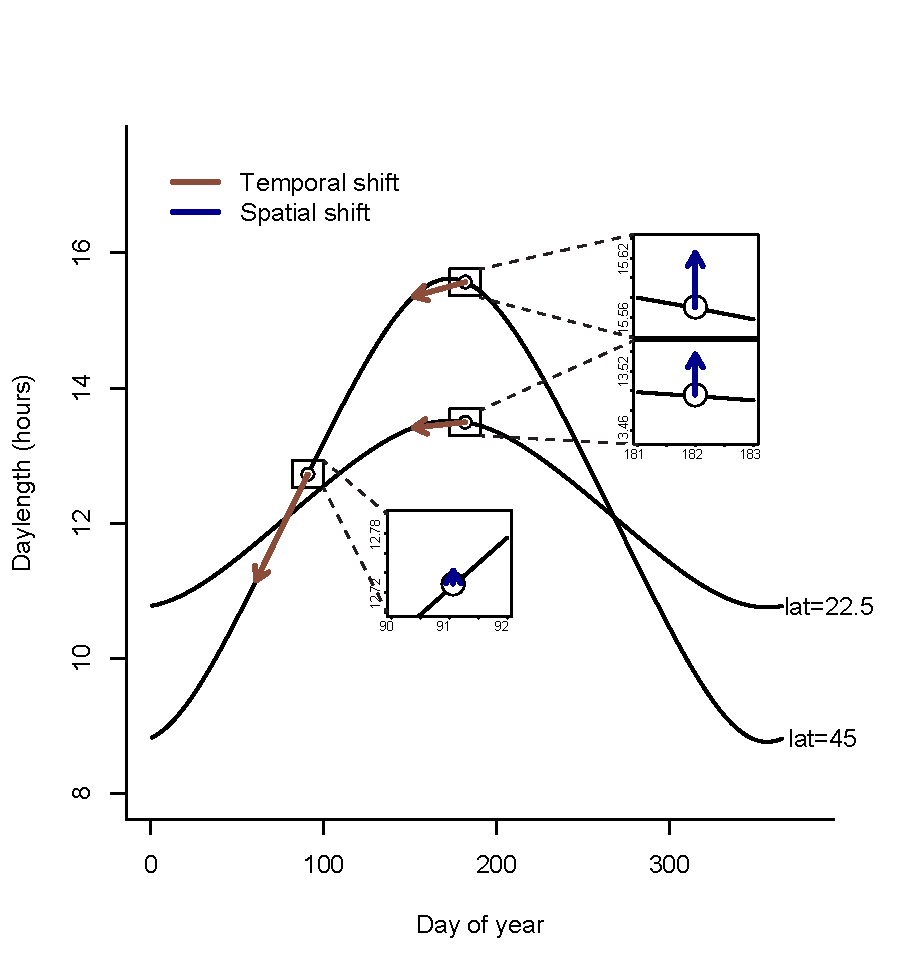
\includegraphics[width=90mm,scale=0.5]{..//..//analyses/photoperiod/figures/photo_spacetime_v2.pdf} \\

%\caption{Figure 1: Photoperiod varies with latitude and by day of year, such that temporal shifts in activity yield larger changes in experienced photoperiod compared with spatial shifts. Here, we show this variation at two latitudes (22.5\degree, 45\degree), using hypothetical spatial and temporal shifts. These shifts,
%which are similar to observed average rates with recent global warming (e.g., \emph{1,5}), highlight the greater magnitude in daylength changes close to the equinox (e.g., day of
%year 91), versus close to the summer solstice (e.g., day of year 182).}
 %\label{fig:condiag}
 %\end{figure}
 
 %\begin{figure}
%\centering
%\includegraphics[width=130mm,scale=0.5]{..//..//analyses/photoperiod/figures/ospree_photopmap_fromblake.jpg} 

%\caption{Figure 2. Experimental photoperiod treatments and their equivalent spatial and temporal shifts for growth chamber experiments that manipulate photoperiod, compiled in a new database (\emph{6}). To calculate the required spatial (lines) or temporal (symbols) shifts for each experiment, we used observed rates with recent warming: 16.9 kilometers per decade (or approximately 1.5 degrees in 100 years) for spatial shifts (\emph{1}) and 2.3 days per decade (or 23 days in 100 years) for temporal shifts (\emph{2}).}
 %\label{fig:photomap}
 %\end{figure}


\end{footnotesize}
\end{letter}
\end{document}
